\documentclass[final]{fhnwreport}       %[mode] = draft or final
                                        %{class} = fhnwreport, article, 
                                        %          report, book, beamer, standalone
%%---Main Packages-----------------------------------------------------------------------
\usepackage[english, ngerman]{babel}	%Mul­tilin­gual sup­port for LaTeX
\usepackage[T1]{fontenc}				%Stan­dard pack­age for se­lect­ing font en­cod­ings
\usepackage[utf8]{inputenc}				%Ac­cept dif­fer­ent in­put en­cod­ings
\usepackage{lmodern}                    %The newer Font-Set
\usepackage{textcomp}					%LaTeX sup­port for the Text Com­pan­ion fonts
\usepackage{caption}					%Customising captions in floating environments
\usepackage{graphicx} 					%En­hanced sup­port for graph­ics
\usepackage{float}						%Im­proved in­ter­face for float­ing ob­jects
\usepackage{ifdraft}                    %Let you check if the doc is in draft mode
\usepackage{enumitem}


%%---Useful Packages---------------------------------------------------------------------
\usepackage{colortbl}	
\usepackage{color}						%Colour control for LaTeX documents
\usepackage[pdftex,dvipsnames,tabl]{xcolor}  %Driver-in­de­pen­dent color ex­ten­sions for LaTeX
\usepackage{csquotes}                   %Simpler quoting with \enquote{}
\usepackage{siunitx} 					%A com­pre­hen­sive (SI) units pack­age
%\usepackage{listings}					%Type­set source code list­ings us­ing LaTeX
\usepackage[bottom]{footmisc}			%A range of foot­note op­tions
\usepackage{footnote}					%Im­prove on LaTeX's foot­note han­dling
\usepackage{verbatim}					%Reim­ple­men­ta­tion of and ex­ten­sions to LaTeX ver­ba­tim
\usepackage[textsize=footnotesize]{todonotes} %Mark­ing things to do in a LaTeX doc­u­ment
\usepackage{titling}					%Control over the typesetting of the \maketitle command
\usepackage[euler]{textgreek}		%Allows to write greek letters without entering math-mode (\textOmega)

%%---Tikz Packages-----------------------------------------------------------------------
\usepackage{standalone}
\usepackage{tikz}
\usepackage{circuitikz}
\usetikzlibrary{arrows}
\usetikzlibrary{calc}
\usetikzlibrary{intersections}

%%---Math Packages-----------------------------------------------------------------------
\usepackage{amsmath}					%AMS math­e­mat­i­cal fa­cil­i­ties for LaTeX
\usepackage{amssymb}					%Type­set­ting symbols (AMS style)

%\usepackage{amstext}
%\usepackage{amsfonts}
%\usepackage{breqn}
%\usepackage{array}						%Ex­tend­ing the ar­ray and tab­u­lar en­vi­ron­ments
%\usepackage{amsthm}					%Type­set­ting the­o­rems (AMS style)

%%---Table Packages----------------------------------------------------------------------
\usepackage{tabularx}					%Tab­u­lars with ad­justable-width columns
%\usepackage{longtable}
%\usepackage{multirow}					%Create tab­u­lar cells span­ning mul­ti­ple rows
\usepackage{multicol}					%In­ter­mix sin­gle and mul­ti­ple columns



%%---PDF / Figure Packages---------------------------------------------------------------
\usepackage{pdfpages}					%In­clude PDF doc­u­ments in LaTeX
%\usepackage{pdflscape}					%Make land­scape pages dis­play as land­scape
%\usepackage{subfig}					    %Fig­ures di­vided into sub­fig­ures

%%---Other Packages----------------------------------------------------------------------
%\usepackage{xargs}                     %De­fine com­mands with many op­tional ar­gu­ments


%%---Bibliography------------------------------------------------------------------------
\usepackage[style=ieee,urldate=comp,backend=biber]{biblatex}
\addbibresource{literature/bibliography.bib}

%%---Main Settings-----------------------------------------------------------------------
\graphicspath{{./graphics/}}			%Defines the graphicspath
\geometry{twoside=false}				    %twoside=false disables the "bookstyle"
\setlength{\marginparwidth}{2cm}
\overfullrule=5em						%Creates a black rule if text goes over the margins => debugging




%%---User Definitions--------------------------------------------------------------------
%%Tabel-Definitions: (requires \usepackage{tabularx})
\newcolumntype{L}[1]{>{\raggedright\arraybackslash}p{#1}}    %column-width and alignment
\newcolumntype{C}[1]{>{\centering\arraybackslash}p{#1}}
\newcolumntype{R}[1]{>{\raggedleft\arraybackslash}p{#1}}
\usepackage{subcaption}


%%---Optional Package Settings-----------------------------------------------------------
%Listings-Settings: (requires \usepackage{listings}) => Example with Matlab Code
%\lstset{language=Matlab,%
%    basicstyle=\footnotesize\ttfamily,
%    breaklines=false,%
%    morekeywords={switch, case, otherwise},
 %   keywordstyle=\color{Blue},%
 %  tabsize=2,
    %morekeywords=[2]{1}, keywordstyle=[2]{\color{black}},
%    identifierstyle=\color{Black},%
%    stringstyle=\color{Purple},
%    commentstyle=\color{Green},%
%    showstringspaces=false,%without this there will be a symbol in the places where there is a space
%    numbers=left,%
%    numberstyle={\tiny \color{black}},% size of the numbers
%    numbersep=9pt, % this defines how far the numbers are from the text
    %emph=[1]{word1, word2,...},emphstyle=[1]\color{red}
%}							

%Hurenkinder und Schusterjungen verhindern (kein Scherz, Google es)
\clubpenalty10000
\widowpenalty10000
\displaywidowpenalty=10000	



%Titel mit Mathematik immer fett drucken
\usepackage{sectsty}
\allsectionsfont{\boldmath}



			                %loads all packages, definitions and settings											
\title{Pflichtenheft}  		        %Project Title
\author{Schenk Kim, Aebi Robin}      				    %Document Type => Technical Report, ...
\date{\today}          				   %Place and Date

\begin{document}

%%---TITLEPAGE---------------------------------------------------------------------------------
\thispagestyle{empty}
%	\ohead{\includegraphics[scale=0.5]{Bilder/Logo_FHNW.jpg}}
	\begin{figure}
		 \vspace*{-\topskip}\vspace*{-\headsep}
		
\includegraphics[scale=1]{graphics/fhnw_ht_logo_de.pdf}
	\end{figure}
	\begin{center}
		\vspace*{2cm}
		{\huge{\textbf{\thetitle}}}\\
		\vspace*{0.5cm}
		
		{\scshape\Large Projekt 5e \\} \Large{\today}
		\vfill
		\begin{normalsize}
			{\begin{tabbing}
%					\textbf{Auftraggeber:} \hspace{5cm}\= Prof. Hans Gysin\\
					
					\\[0.8cm]
					\textbf{Dozent:} \hspace{5cm}
					\=Prof. Dr. Schleuniger, Pascal\\
					
					
					\\[0.4cm]
%					\textbf{Projektleiter:} \>Fabian von Büren\\
%					\\[0.4cm]
					
					\textbf{Team:} \>Aebi, Robin \\ \>Schenk, Kim \\
					\\[0.8cm]
					\textbf{Studiengang:} \>Elektro- und Informationstechnik
					\\[0.8cm]	\textbf{Semester:} \>Herbstsemester 2019
			\end{tabbing}}
		\end{normalsize}
		\vfill
	\end{center}
\clearpage

%%---TABLE OF CONTENTS-------------------------------------------------------------------
\pagenumbering{Roman}		
\selectlanguage{ngerman}				%ngerman or english
\tableofcontents
\clearpage

%%---TEXT--------------------------------------------------------------------------------
\pagenumbering{arabic}
\clearpage
\section{Einleitung}\label{sec:Einleitung}
Das Organisatorische Pflichtenheft beinhaltet viele verschiedene Teilschritte, welche die Rahmenbedingungen definieren. In diesem werden die Projektziele, Lieferobjekte sowie die die Meilensteine festgelegt. Ausserdem beinhaltet es einen detaillierten Projektstrukturplan, welcher Arbeitspakete und den Zeitplan enthält.

\subsection{Ausgangslage}\label{subsec:Ausgangslage}

Bei einer gelungenen Gartenparty dürfen erfrischende Getränke nicht fehlen. Das Problem ist jedoch, dass kaum einer weiss, wie Cocktails gemischt werden und keiner Lust hat den ganzen Abend Barmann/Frau zu spielen. Hier soll nun die Cocktailmaschine für zu Hause Abhilfe schaffen und somit eine gelungene Gartenparty garantieren.

Es soll eine automatische Cocktail-Maschine entwickelt werden. Die Benutzer können wahlweise über eine Handy-App oder ein Display ihr Cocktailglas individuell konfigurieren. Die Cocktail-Maschine erkennt das Cocktailglas und stellt anhand der gespeicherten Serverdaten das gewünschte Getränk zusammen. 
 
\newpage
\subsection{Projektziele}\label{subsec:Projektziele}

\subsubsection{Pflichtziele}\label{sec:Pflichtziele}

\begin{enumerate}

\item \underline{\textbf{Detailkonzept}}\mbox{}\\

Das Detailkonzept wird so ausgearbeitet, dass alle dazugekommenen Komponenten ebenfalls darin enthalten sind. Daraus ergibt sich folgende Liste:\\

Bestehend:
\begin{itemize}
\item Speisungen (48V, 12V, 5V, 3.3V)
\item Motor
\item ABN-Encoder
\item Endschalter
\item Motorentreiber
\item Gatetreiber
\item Durchflussmessungen
\item Pumpen
\item Display
\item Mikrocontroller\\
\end{itemize}

Dazugekommen:

\begin{itemize}
\item USB
\item Wirelessmodul
\item RFID
\item Beleuchtung\\
\end{itemize}

\item \underline{\textbf{Design der Leiterplatte}}\mbox{}\\

Beinhaltet alle Teile des Detailkonzeptes. Für das WIFI-, RFID- und Motorentreiber-Modul wird ein Development-Board verwendet. Zusätzlich zum WIFI- und RFID-Modul wird eine eigen gelayoutete Variante miteinbezogen, welche bei genügend Kapazität implementiert wird anstelle des Moduls.\\

\item \underline{\textbf{Mechanischer Aufbau der Maschine inkl. Achsensystem}}\mbox{}\\

Der mechanische Aufbau der Maschine beinhaltet folgende Teile:

\textbullet Rahmen \newline
\textbullet Getränkehalterung \newline
\textbullet Flüssigkeitsbeförderung \newline
\textbullet Gehäuse für Elektronik \newline
\textbullet Befestigung für Display \newline
\textbullet Glasbeförderungssystem \newline
\textbullet Überlaufwanne \newline
\textbullet Beleuchtung\\
\newpage

\item \underline{\textbf{Regler Parametrierung des Achsensystems}}\mbox{}\\

Die Regelung des Achsensystems wird mit dem TMC4671 gewährleistet. Die Regler werden so ausgelegt, dass das Glas während dem Fahren nicht überläuft. Die Bewegungsgeschwindigkeit soll jedoch auch schnell genug sein, dass der Drink in unter einer Minute hergestellt wird.\\

\item \underline{\textbf{Bediensoftware}}\mbox{}\\

Die Bediensoftware auf dem Mikrocontroller ermöglicht dem Benutzer folgende Eingaben:\\
\begin{itemize}

\item Getränkeliste
\item Wo steht welches Getränk
\item Infos zum Getränk
\item Auswahl Zubereitung 0.3l oder 0.5l
\item Eingabe eigener Getränke
\item Speichern von Getränkefavoriten
\item Nachfüllen des Lieblingsgetränks mittels RFID
\item Reinigungsmodus\\
\end{itemize}

Über einen Web-Server kann der User die selben Anwendungen in abgespeckter Version auswählen.\\

\item \underline{\textbf{Funktionstest und Analyse bezüglich der Skalierbarkeit}}\mbox{}\\
			
In einer ersten Phase wird der Print in Betrieb genommen. Dies bedeutet, dass die einzelnen Systeme mit Sonderprogrammen auf ihre Funktion geprüft werden. Dies beinhaltet die Systeme des Detailkonzeptes.\\

In einer zweiten Phase wird die Maschine auf ihre Funktion gepfüft. Dies soll die Funktionen beinhalten, welche in der Bediensoftware aufgelistet sind.\\
			
			 
\item \underline{\textbf{Software}}\mbox{}\\

Die Software für den Mikrocontroller soll in C geschrieben sein. 
			
Für das ESP wird vorerst Arduino verwendet.
			
\end{enumerate}	
\newpage
\subsubsection{Wunschziele}\label{sec:Wunschziele}

\begin{enumerate}

\item \underline{\textbf{Lichtkonzept}}\mbox{}\\

Die Maschine bietet einen gewissen Showeffekt. Dazu wird ein LED-Streifen montiert, welcher die Maschine beleuchtet. Für die Beleuchtung werden RGB-LED's verwendet, was eine entsprechende Ansteuerung Hard- und Softwareseitig erfordert.\\

\item \underline{\textbf{Software}}\mbox{}\\

Die Software für das ESP soll in C geschrieben sein.
\end{enumerate}

\newpage

\subsection{Projektmanagement, Kommunikation, Abgabetermine, Bewertung}

Das Projekt soll von einem schlanken, ergebnisorientierten Projektmanagement begleitet werden. 
Die betreuenden Dozenten sollen periodisch (mind. alle 3 Wochen) über den Stand der Arbeiten sowie allfälliger Abweichungen zum Pflichtenheft und Projektplan informiert werden.
Es finden mindestens folgende Meetings statt: Kickoffmeeting, Besprechung Pflichtenheft/Projektvereinbarung sowie Schlusspräsentation/Verteidigung. 
Bei Bedarf können mehr Meetings durchgeführt werden.
Bezüglich Verteidigung und Bewertung gelten die Vorgaben und Richtlinien der FHNW, Hochschule für Technik.

\newpage

\subsection{Lieferobjekte}\label{subsec:Lieferobjekte}
\begin{itemize}

\item \textbf{Projektvereinbarung}\\

Per Mail,

An Projektcoach,

Bis 05.03.2020. \\

\item \textbf{Projektunterlagen (Fachbericht, Hardware, Programmcode, Schemas etc.)}\\

Per Mail, Physisch, auf USB,

An Projektcoach,

Bis 15.08.2020.\\

\item \textbf{Präsentation und Verteidigung}\\

Meeting,

In Anwesenheit von Projektcoach und Experten,

Zischen 31.08.20 und 12.09.2020.\\

\item \textbf{Fact Sheet}\\

Im LaTeX-Format inkl. Bilder und PDF (gesamter Ordner als zip-Datei),

Upload über die Projektdatenbank,

Bis spätestens 19.09.2020.\\

\item \textbf{Poster}\\

Auf Papier für Projektausstellung,

Im pptx-Format und im pdf-Format (beides in einer zip-Datei),

Upload über die Projektdatenbank,

Bis 14.08.2020.\\

\item \textbf{Räumung des Arbeitsplatzes}\\

Bis spätestens 12.09.2020


\end{itemize}	

\pagebreak

%\input{sections/1_0_Organisationsstruktur}
%\pagebreak

\newpage

\begin{landscape}

\section{Projektstrukturplan}\label{sec:Projektstrukturplan}
In Projektstrukturplan sind die verschiedenen Meilensteine und die genaue Einteilung der Personenstunden im Verlauf des Semesters ersichtlich.

\subsection{Arbeitspakete und Zeitplan}\label{subsec:Arbeitspakete_und_Zeitplan}

\begin{figure}[h]
   \centering
   \noindent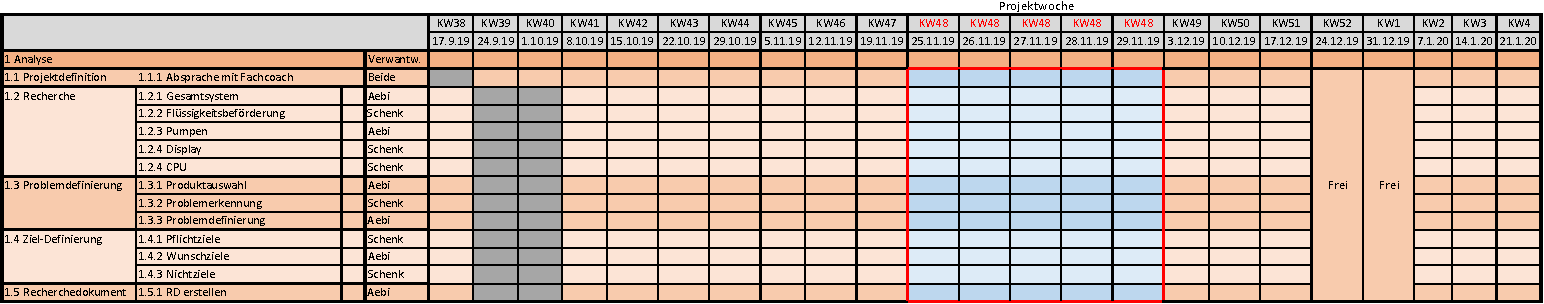
\includegraphics[width=\linewidth,keepaspectratio]{graphics/Analyse.pdf}
%   \caption[Beispielbild]{Beispielbild}
   \label{pic:Analyse}
\end{figure}

\begin{figure}[h]
   \centering
   \noindent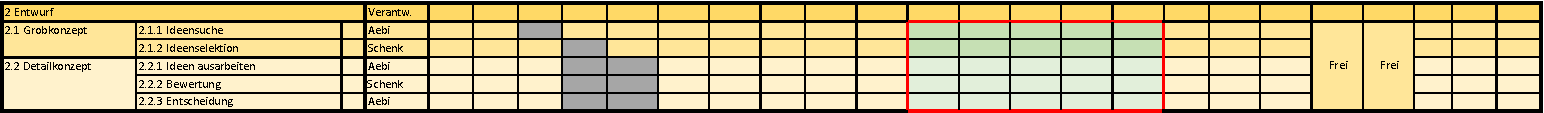
\includegraphics[width=\linewidth,keepaspectratio]{graphics/Entwurf.pdf}
%   \caption[Beispielbild]{Beispielbild}
   \label{pic:Entwurf}
\end{figure}

\begin{figure}[h]
   \centering
   \noindent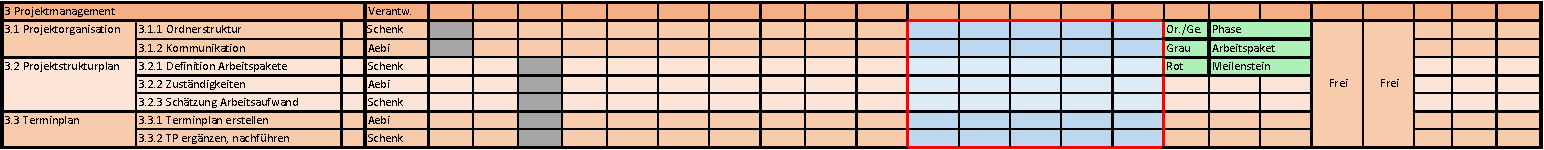
\includegraphics[width=\linewidth,height=.9\textheight,keepaspectratio]{graphics/Projektmanagemant.pdf}
%   \caption[Beispielbild]{Beispielbild}
   \label{pic:Projektmanagement}
\end{figure}
\vfill
\clearpage
\begin{figure}[h]
   \centering
   \noindent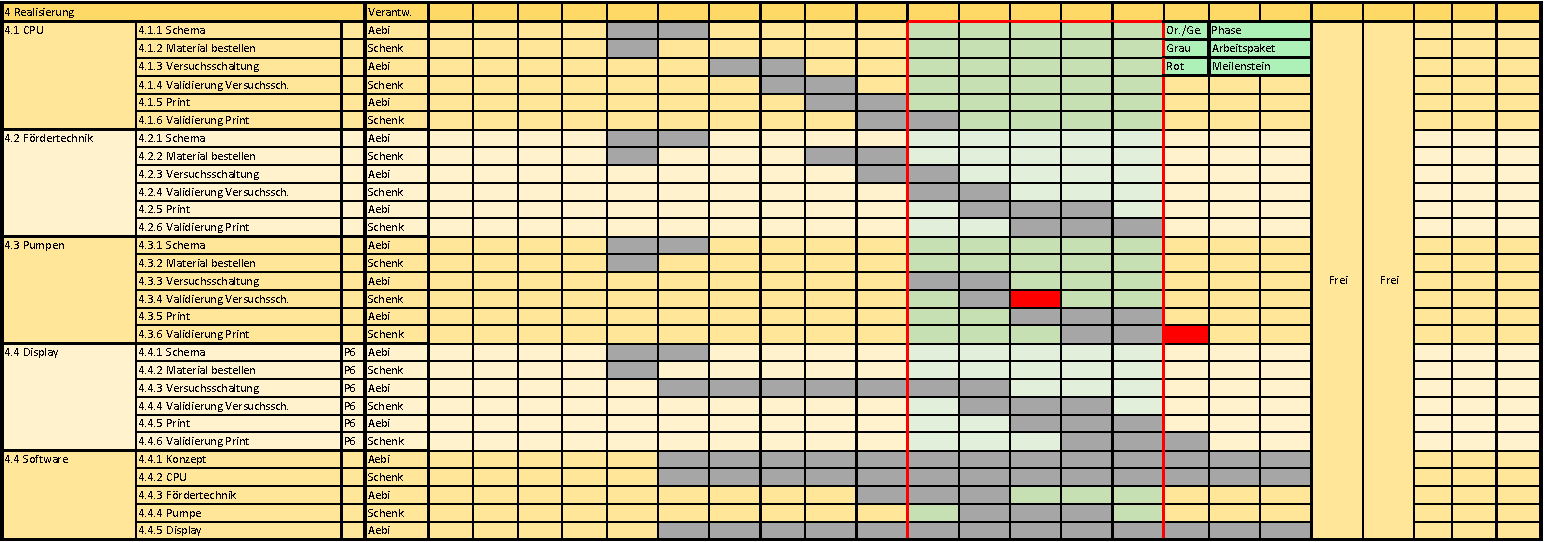
\includegraphics[width=\linewidth,keepaspectratio]{graphics/Realisierung.pdf}
%   \caption[Beispielbild]{Beispielbild}
   \label{pic:Realisierung}
\end{figure}
\clearpage
\subsection{Meilensteine}\label{subsec:Meilensteine}
 \begin{figure}[h]
   \centering
   \noindent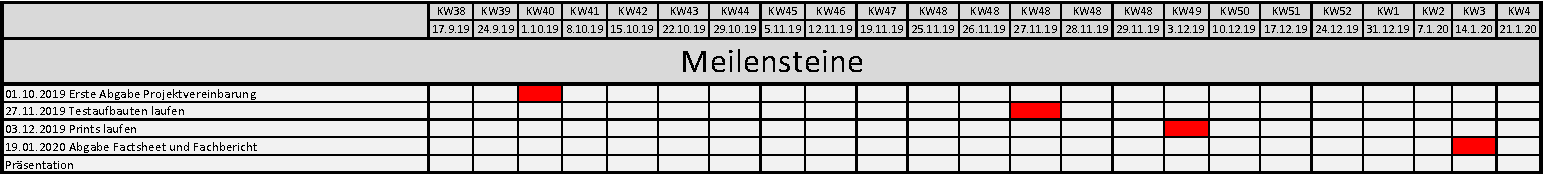
\includegraphics[width=\linewidth,height=.9\textheight,keepaspectratio]{graphics/Meilensteine.pdf}
%   \caption[Beispielbild]{Beispielbild}
   \label{pic:Meilensteine}
\end{figure}
\vfill
\end{landscape}
\pagebreak

%\input{sections/3_0_Projektbudget}
%\pagebreak

%\input{sections/4_0_Kommunikationskonzept}
%\pagebreak

%\input{sections/5_0_Risikomanagement}
%\pagebreak

\clearpage
\section{Projektvereinbarung}\label{sec:Projektvereinbarung}
	\begin{tabbing}
		\textbf{Betreuender Dozent}\\[0.2cm]
		Prof. Dr. Schleuniger, Pascal \\[0.2cm]
		Ort, Datum: \hspace{5cm}\=Unterschrift:
		\\[0.5cm]----------------------------- \>-----------------------------
		\\[0.5cm]
		\textbf{Student}\\[0.2cm]
		Aebi, Robin\\[0.2cm]
		Ort, Datum: \>Unterschrift:
		\\[0.5cm]----------------------------- \>-----------------------------
		\\[0.5cm]
		\textbf{Student}\\[0.2cm]
		Schenk, Kim\\[0.2cm]
		Ort, Datum: \>Unterschrift:
		\\[0.5cm]----------------------------- \>-----------------------------
	\end{tabbing}
	
	\clearpage






\clearpage
%%---BIBLIOGRAPHY------------------------------------------------------------------------
{\sloppypar
\printbibliography
\label{sec:lit}
%\selectlanguage{ngerman}				%ngerman or english
%\printbibliography
}


%%---NOTES for DEBUG---------------------------------------------------------------------
\ifdraft{%Do this only if mode=draft
%%requires \usepackage{todonotes})
\newpage
\listoftodos[\section{Todo-Notes}]
\clearpage
}
{%Do this only if mode=final
}

\end{document}
